
\chapter{Robotic Platform for Mobile Manipulation}

This chapter will describe the robotic platform used for the project, specifically the hardware components.
The platform is composed of a mobile robot base, a robotic arm manipulator, sensors and perception systems, 
a soft gripper actuator, and 3D-printed mounts.
The chapter will also discuss the issues faced during the development of the platform.

\section{Mobile Robot Platform}

The mobile robot used for the Thesis project is an \textit{AgileX Scout 2.0} robot. 
This robot is a skid-steering robot, suitable for outdoor and indoor environments. 
Designed for robotics research and development, the Scout 2.0 is an unmanned ground vehicle (UGV). 
This autonomous mobile robot is CE-certified and offers a robust mechanical design along with capable mobility performance. 
Built to endure diverse conditions, Scout 2.0 features rugged materials and protective casings, ensuring longevity
and reliability during missions. SCOUT 2.0 offers aluminum T-slot rails for secure mounting of external sensors or kits. 
On these rails, a variety of sensors, computers or other devices are mounted, allowing the creation of a mobile robotic platform
for a wide range of applications, and without relying on power cables to the wall, thanks to its onboard battery system.
It supports CAN bus protocol for connections and provides open-source SDK and software resources for expanded capabilities.
Its maximum speed is $1.5 m/s$, and it can carry a payload of $50$ kg. 
The robot is powered by a 24V battery, which provides a range of $15$ km maximum. 
The robot is controlled by a ROS-based software system, which allows the control of the robot's speed using a ROS topic
and receiving odometry data from the robot's encoders.

%Add the image of the robot
\begin{figure}[ht]
	\centering
	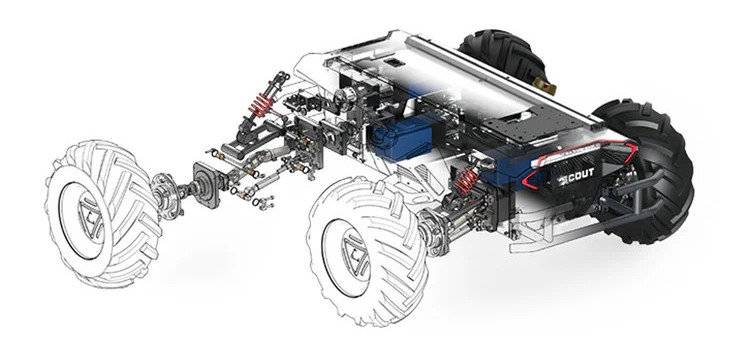
\includegraphics[width=1\textwidth]{chapter3_01.jpg}
	\captionsetup{width=1\linewidth}
	\caption{SCOUT employs 200W brushless servo motors to drive each wheel independently. 
    Its double-wishbone suspension with shock absorbers ensures stability on rough terrain, 
    enabling it to tackle obstacles up to 10cm tall effortlessly.}.
	\label{fig:c3_img01}
\end{figure}

The robot's internal battery is capable of powering all the sensors and computational
units that are mounted. To meet the specific voltage and current requirements of these devices, 
two DC/DC converters are employed:
- one DC/DC converter with an output voltage of 12V at a maximum of 15A for the on-board computer, router, and switch
- one DC/DC converter with an output voltage of 24V at a maximum of 5A for the LiDAR sensor.

% Add image of DC/DC converters
\begin{figure}[ht]
    \centering
    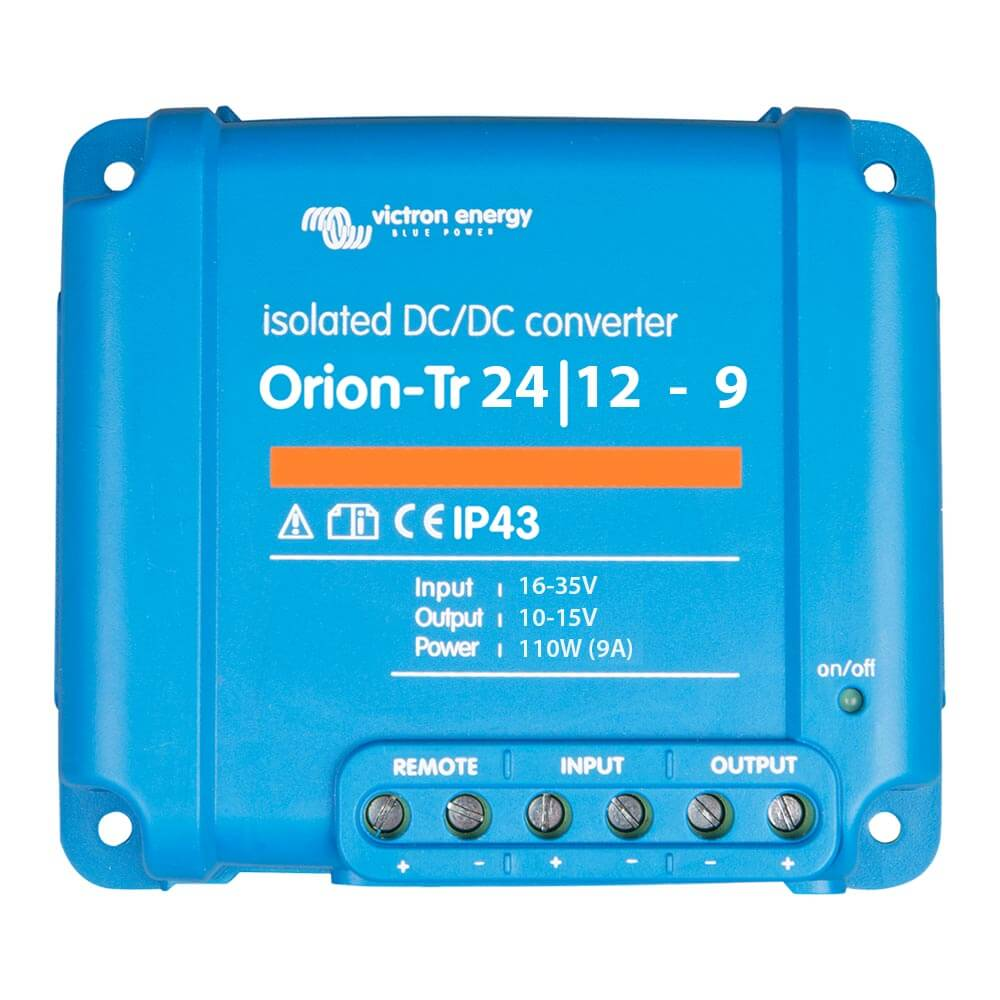
\includegraphics[width=0.5\textwidth]{chapter3_03.jpg}
    \captionsetup{width=1\linewidth}
    \caption{DC/DC converter used to power the robot's sensors and computer}.
    \label{fig:c3_img03}
\end{figure}

On the mobile robot, an \textit{Intel NUC 12} computer is mounted. This computer is used for running all the control
software and the perception algorithms. The computer is connected to a switch, which is used to connect
the computer to the robot's control system and all the sensors and electronic devices mounted on the robot.
The computer is also connected to a router, which is used to connect the computer to the laboratory's network
and the internet. This allows the robot to be controlled remotely via a remote desktop connection.
This computer has the following technical specifications:

\begin{itemize}
    \item Intel Core i7-12700H CPU
    \item 32GB DDR4 RAM
    \item 1TB NVMe SSD
    \item Intel Iris Xe Graphics
    \item Kubuntu 22.04 operating system
\end{itemize}

% Add the image of the computer
\begin{figure}[ht]
    \centering
    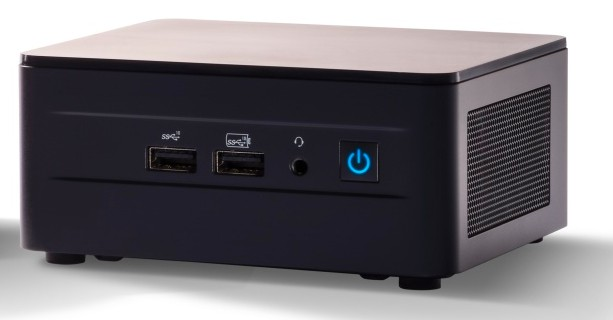
\includegraphics[width=0.6\textwidth]{chapter3_02.jpg}
    \captionsetup{width=1\linewidth}
    \caption{Intel NUC 12 computer mounted on the robot}.
    \label{fig:c3_img02}
\end{figure}

The robot is equipped with an \textit{TP-Link Archer MR200} router and a \textit{Netgear GS108} switch.
The router is used to connect the robot to the laboratory's network and the internet. The router was necessary to
establish a remote connection from a personal laptop to the robot's computer, allowing the control and monitoring
of the robot from a remote location. This was essential for the development of the project, as it allowed me to
work safely with the robot, ensuring that everything was working smoothly and stopping the system in case of any
unexpected behavior or software crashes and malfunctions.

The switch is used to connect the robot's computer to the robot's control system and all the sensors
and electronic devices mounted on the robot. The switch is connected to the router, allowing the robot's computer
to communicate with the laboratory's network and the internet. The robotic arm manipulator is also connected to the switch,
allowing the robot's computer to control the manipulator and receive data from its motors' encoders. 
The LiDAR is connected to the switch, allowing the robot's computer to receive pointcloud data from the LiDAR sensor,
at a fast transmission rate.
 
\section{Robotic Arm Manipulator}

The robotic arm manipulator used for the Thesis project is a \textit{Igus ReBeL 6-DoF} robotic arm.
This robotic arm is a lightweight, compact, and affordable robotic arm, suitable for research and development
in robotics. It is produced by the German company Igus, which specializes in the production of robotic components
for low-cost automation. The robotic arm is composed of six joints, each driven by a DC motor with an integrated encoder.
The outer contour and mechanical components of the ReBeL utilize Igus® plastic polymers, making it particularly inexpensive
and the lightest cobot on the market. Its lightweight and compact design makes it suitable for mounting on top
of mobile robot platforms, such as the SCOUT 2.0 robot. The maximum payload of the arm is $2$ kg, which is more than enough
for the project's requirements. The weight is $8.2$ kg, which is light enough to be carried around by the mobile robot base,
without affecting the robot's mobility and stability.

The \textbf{advantages} of the ReBeL robotic arm are:

\begin{itemize}
    \item Lightweight, sleek and compact design
    \item Plastic arm, inexpensive and cost-effective
    \item Easy to install and operate
    \item Plug and play proprietary control system, or open-source control option
\end{itemize}

The \textbf{disadvantages} of the ReBeL robotic arm are:
\begin{itemize}
    \item Limited reach and workspace due to the joints' design and physical constraints
    \item Limited precision and repeatability
    \item The plastic gear components are not as durable and reliable as metal components
\end{itemize}

% Add the of the robotic arm
\begin{figure}[ht]
    \centering
    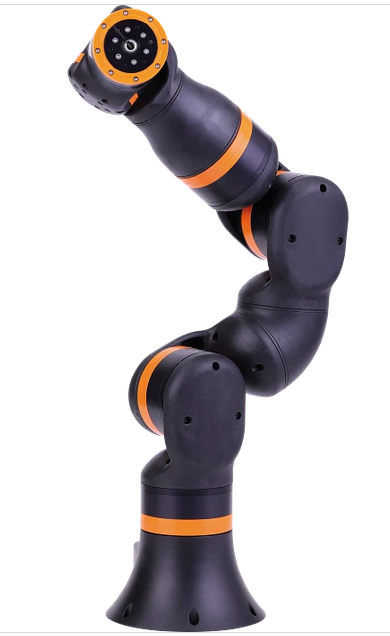
\includegraphics[width=0.3\textwidth]{chapter3_04.png}
    \captionsetup{width=1\linewidth}
    \caption{Igus ReBeL 6-DoF robotic arm}.
    \label{fig:c3_img04}
\end{figure}

This robotic arm was the ideal choice for the project since the open-source control option allowed me to develop
the control software for the arm, based on ROS2 software packages. The lightweight and compact design made it suitable
for mounting on top of the SCOUT 2.0 robot, without affecting the robot's mobility and performance. 
The arm's easy installation and operation allowed me to quickly set up the arm and start developing the control software
and perception algorithms for the project.

% Add the image of the robotic arm software
\begin{figure}[ht]
    \centering
    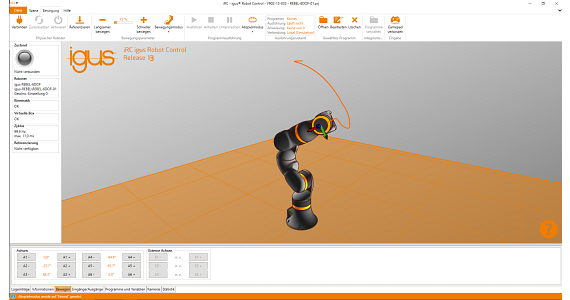
\includegraphics[width=0.8\textwidth]{chapter3_05.png}
    \captionsetup{width=1\linewidth}
    \caption{Igus ReBeL proprietary control software interface}.
    \label{fig:c3_img05}
\end{figure}

\subsection*{Issues with Igus Rebel motors' encoders and calibration}

Throughout the development of the project, I encountered several issues with the Igus ReBeL robotic arm.
The issues arose when the arm's motors' encoders were not providing accurate position data to the control software.
This caused the arm not to move to the defined joint positions with an accuracy of the end effector of $\pm 0.1mm$,
as specified by the manufacturer in the technical documentation.
This was mainly due to both the calibration of the motors' encoders and the plastic gear components' backlash and play.

The backlash and play in the gear components caused the arm's joints to have a certain amount of free movement before the motor
started to move the joint. This free movement caused the arm's joints to be in an incorrect position, which was not detected
by the motor's encoders. This resulted in the arm jiggling and vibrating when moving to a new joint position, and not reaching
the desired position with a smooth velocity profile.

Furthermore, the main issue encountered was the calibration of the motors' encoders. This problem slowed down the development
of the project since the software solutions for the calibration of the encoders and the digital zeroing of the joints were not
successful in providing a working solution for the arm's accurate positioning. The calibration of the encoders was necessary
to provide accurate position data to the control software, allowing the arm to move to the desired joint positions with high
precision. The problem encountered was that the software for the automatic calibration of the motor controllers did not work
as expected, resulting in errors and faulty calibration of the encoders. The only solution was to replace the entire robot
arm with a new one, correctly calibrated by the manufacturer.

\section{Sensors and Perception}

The mobile robot platform is equipped with several sensors and perception systems, which are essential for the project's
objectives. The sensors and perception systems are used for mapping and localization, obstacle avoidance, object detection
and recognition, and manipulation tasks. 

\subsection{3D LiDAR Sensor}

The main sensor for environment perception for localization and navigation is mounted on the robot's T-slot rails.
The sensor is a \textit{Ouster OS1-64} LiDAR sensor.
The OS1 offers clean, dense data across its entire field of view for accurate perception and crisp detail in industrial,
automotive, robotics, and mapping applications.
This sensor is a 64-plane LiDAR sensor, capable of providing a 360-degree field of view with a range of $120$ meters. 
The sensor has a resolution of $\pm 0.1cm$ and a stable scan rate of $10 Hz$ at $1024$ points resolution.
The vertical and horizontal scan resolution are $\pm 0.01$°.
Its minimum range of $0.5$ meters makes it suitable for indoor environments, while its maximum range of $120$ meters
makes it suitable also for outdoor environments.
This sensor was employed to create maps of the environments and also to localize the robot within the environment.
It proved also useful for dynamic obstacle avoidance, thanks to its high resolution and scan rate.

%insert image of the LiDAR sensor
\begin{figure}[ht]
    \centering
    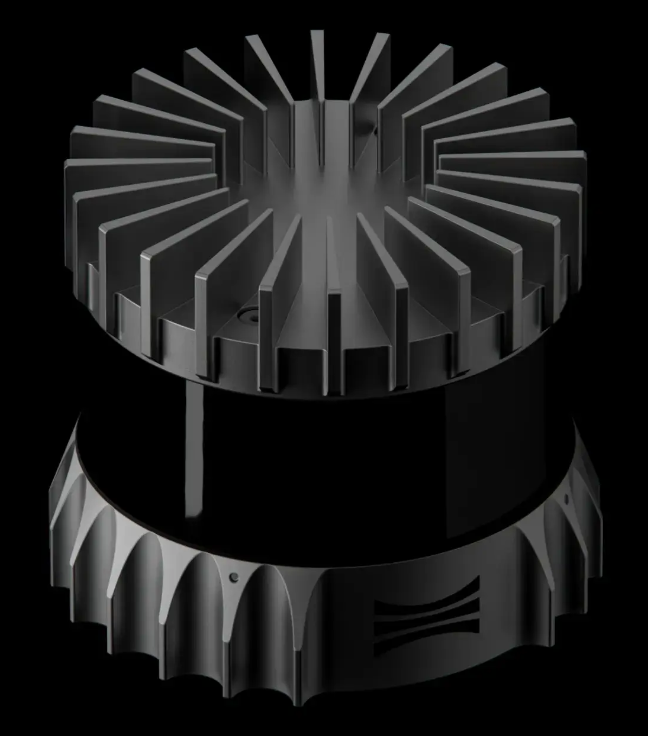
\includegraphics[width=0.5\textwidth]{chapter3_06.png}
    \captionsetup{width=1\linewidth}
    \caption{Ouster OS1-64 LiDAR sensor}.
    \label{fig:c3_img06}
\end{figure}

\subsection*{Issues with LiDAR low frequency}

Throughout the development of the project, I encountered several issues with the autonomous navigation stack.
Sometimes the software crashed at random times, unpredictably, and without any apparent reason.
Some other times the dynamic obstacle avoidance algorithm did not work as expected, causing the robot to collide
with obstacles that were not perceived by the LiDAR sensor in the surrounding environment.
Overall, the robot's navigation stack was not reliable and robust, which was a significant issue for the project's development,
especially for the autonomous navigation tasks in the laboratory's environment (cluttered and dynamic).

After many trials and tests, my supervisor and I discovered that the LiDAR pointcloud data's low and unreliable frequency
was the main cause of all these problems. The LiDAR sensor works at a nominal frequency of $10$Hz. 
The LiDAR sensor was not providing a stable scan rate of $10$Hz, but it was fluctuating between $3$Hz and $8$Hz, 
and only in a few cases, it was able to provide the nominal $10$Hz scan rate.
Once we discovered the source of the problem and ensured that the LiDAR sensor was working correctly
(meaning that the sensor was not malfunctioning or working at a lower but valid data rate), 
we tried to find the culprit of the low and unreliable frequency of the LiDAR sensor.

After many attempts, I found out the cause of the problem: the culprit was the router used to connect the robot's computer
to the laboratory's network and the internet and the DDS (\textit{Data Distribution Service}) middleware used 
internally by ROS2 for the communication between the nodes in a local network. Basically, the DDS middleware
was configured to broadcast all ROS2 packets and data streams to the laboratory's network, causing delays in the transmission
and packet loss, as the network was not able to handle the high-frequency and heavy-weight data streams of the LiDAR sensor.
In fact, by just unplugging the router from the robot's computer, the LiDAR sensor was able to provide a stable scan rate
of $10$Hz, without any fluctuations or drops in the frequency, since no broadcast packets were sent to the network.
Since the router was necessary for the remote control and monitoring, it was simply just not an option
to unplug it from the robot's computer.

For the correct operation of the robot's localization and obstacle 
avoidance algorithms, it is fundamental that the LiDAR sensor works at a stable frequency, 
without any fluctuations or drops in the scan rate. This requirement is essential because these algorithms rely on the
coherent and continuous data stream for time interpolation and filtering of the pointcloud data.
This is why the LiDAR sensor's low and unreliable frequency was causing the software to crash and malfunction.

The solution was to configure properly the DDS middleware to ensure that all ROS-related nodes and data streams
were handled inside the robot's computer only, and not going through the router and the laboratory's network.
Having the data streams in the local machine only, ensured that the LiDAR sensor's data was not distributed 
among the network, causing delays in the transmission and packet loss, which were the main causes of the low and unreliable
frequency of the LiDAR sensor. Furthermore, we configured ROS2 to use the \textit{Cyclone DDS} middleware, which is a lightweight
and fast DDS implementation, suitable for real-time and high-frequency data streams. This DDS implementation was able to handle
heavy-weight data packets at high frequencies, ensuring that the LiDAR sensor's data was transmitted and received correctly
in its entirety, without any losses or delays in the transmission.

After this configuration, the LiDAR sensor was able to provide a stable scan rate of $10$Hz,
and the software stack was working correctly, without any crashes or malfunctions.
Furthermore, I was also able to test the LiDAR sensor at a higher frequency of $20$Hz, 
with lower resolution, and it was working fine and stable.
This solution was essential also for the correct operation of the IMU sensor for the SLAM algorithm, which required
a stable and continuous data stream of the LiDAR at the moment of startup of the sensor in the software stack. Before the 
fix of the LiDAR sensor's frequency, the IMU sensor was not able to start correctly, due to the lack of data
from the LiDAR sensor, and the computed odometry data was drifting too much to be useful.
Many other algorithms and software benefitted from this fix. The robot's navigation stack was now reliable and robust,
and the autonomous navigation tasks were working correctly and smoothly.

\subsection{RGB-D Stereo Camera Sensor}

The robotic arm is equipped with a \textit{Intel Realsense D435} RGB-D stereo camera sensor.
This camera is mounted on the \textit{wrist} of the robotic arm, allowing the camera to move with the arm's end effector.
The camera is used for object detection and recognition, and also for Aruco markers detection and pose estimation.
This is the camera of choice for robotic applications, as it provides both RGB and depth images, which are essential
for perception tasks in robotics. The camera is also lightweight and compact, making it suitable for mounting on the robotic arm.

The Intel RealSense D435 is a stereo depth camera that is designed for capturing RGB and depth images.
The camera is equipped with a global shutter and a rolling shutter, which allows it to capture images with a resolution
of $1920\times1080$ pixels at $30$ frames per second, even though the ROS2 driver provided by Intel reduces the resolution
to $640\times480$ pixels at $30$ frames per second. The camera has a field of view of $85.2$° horizontal, $58$° vertical,
and $94$° diagonal. The depth camera works within a range of $0.3$ meters to $3$ meters while maintaining 
high accuracy and precision. 

\subsection*{Issues with Intel Realsense calibration}

The camera provided by the laboratory was not calibrated correctly, especially the depth estimations were not accurate.
In fact, the depth images provided depth estimations that were not consistent with the real-world distances of the objects
in the environment. I was able to discover such issues when I started using the camera's depth sensor for the perception
tasks of the project. I realized that the estimated distance from the camera and the Aruco markers (distance estimated
using geometrical calculations and the camera's intrinsic parameters) was not consistent with the estimated distance
to the marker provided by the camera's depth sensor. This inconsistency was due to the camera's depth sensor not being
calibrated correctly.

This issue was critical for the project, as the depth sensor was used for many perception algorithms.
I managed to solve this issue by calibrating the camera's depth sensor using the proprietary software provided by Intel.
The calibration process was straightforward and required a few minutes to complete, even though many trials were needed
to find the best possible calibration parameters. Two calibration procedures were carried out:

\begin{itemize}
    \item \textbf{Intrinsic parameters calibration}: this calibration process was used to calibrate the camera's 
    intrinsic parameters,
    such as the focal length, principal point, and distortion coefficients. This calibration was necessary to correct
    the distortion of the images and to provide accurate depth estimations from the RGB sensor. The calibration process
    required the camera to capture a series of images of a calibration pattern (checkerboard pattern) from different angles
    and distances. The calibration software then used these images to estimate the intrinsic parameters of the camera.
    \item \textbf{Depth sensor calibration}: this calibration process required the camera to capture a series of
    depth images of a calibration sheet, which was a flat surface with known distances between the points. The calibration
    software then used these depth images to estimate the depth sensor's parameters, such as the depth scale factor
    and the depth offset. These parameters were necessary to correct the depth estimations of the camera's depth sensor.
\end{itemize}

After the calibration process, the camera's depth sensor was providing accurate and consistent depth estimations,
which were consistent with the real-world distances of the objects in the environment.

\section{Soft Gripper Actuator}

\section{3D Printed Mounts Design}

\subsection*{Issues with the laboratory's 3D printer}

\section{Batteries and Power Management}